\documentclass[12pt,english,dvipsnames,aspectratio=169,handout]{beamer}\usepackage[]{graphicx}\usepackage[]{xcolor}
% maxwidth is the original width if it is less than linewidth
% otherwise use linewidth (to make sure the graphics do not exceed the margin)
\makeatletter
\def\maxwidth{ %
  \ifdim\Gin@nat@width>\linewidth
    \linewidth
  \else
    \Gin@nat@width
  \fi
}
\makeatother

\definecolor{fgcolor}{rgb}{0.345, 0.345, 0.345}
\newcommand{\hlnum}[1]{\textcolor[rgb]{0.686,0.059,0.569}{#1}}%
\newcommand{\hlstr}[1]{\textcolor[rgb]{0.192,0.494,0.8}{#1}}%
\newcommand{\hlcom}[1]{\textcolor[rgb]{0.678,0.584,0.686}{\textit{#1}}}%
\newcommand{\hlopt}[1]{\textcolor[rgb]{0,0,0}{#1}}%
\newcommand{\hlstd}[1]{\textcolor[rgb]{0.345,0.345,0.345}{#1}}%
\newcommand{\hlkwa}[1]{\textcolor[rgb]{0.161,0.373,0.58}{\textbf{#1}}}%
\newcommand{\hlkwb}[1]{\textcolor[rgb]{0.69,0.353,0.396}{#1}}%
\newcommand{\hlkwc}[1]{\textcolor[rgb]{0.333,0.667,0.333}{#1}}%
\newcommand{\hlkwd}[1]{\textcolor[rgb]{0.737,0.353,0.396}{\textbf{#1}}}%
\let\hlipl\hlkwb

\usepackage{framed}
\makeatletter
\newenvironment{kframe}{%
 \def\at@end@of@kframe{}%
 \ifinner\ifhmode%
  \def\at@end@of@kframe{\end{minipage}}%
  \begin{minipage}{\columnwidth}%
 \fi\fi%
 \def\FrameCommand##1{\hskip\@totalleftmargin \hskip-\fboxsep
 \colorbox{shadecolor}{##1}\hskip-\fboxsep
     % There is no \\@totalrightmargin, so:
     \hskip-\linewidth \hskip-\@totalleftmargin \hskip\columnwidth}%
 \MakeFramed {\advance\hsize-\width
   \@totalleftmargin\z@ \linewidth\hsize
   \@setminipage}}%
 {\par\unskip\endMakeFramed%
 \at@end@of@kframe}
\makeatother

\definecolor{shadecolor}{rgb}{.97, .97, .97}
\definecolor{messagecolor}{rgb}{0, 0, 0}
\definecolor{warningcolor}{rgb}{1, 0, 1}
\definecolor{errorcolor}{rgb}{1, 0, 0}
\newenvironment{knitrout}{}{} % an empty environment to be redefined in TeX

\usepackage{alltt}
\usepackage{fontspec}
\setsansfont[Mapping=tex-text]{Fira Sans}
\setcounter{secnumdepth}{4}
\setcounter{tocdepth}{4}
\usepackage[normalem]{ulem}
\usepackage[T1]{fontenc}
\usepackage[utf8]{inputenc}
\usepackage{dcolumn}
\usepackage{booktabs}
\usepackage{bm}
\usepackage{setspace}
\makeatletter
\usetheme{metropolis}
\setbeamertemplate{frame footer}{Bosancianu | Schaub | Hertie School}
\setbeamerfont{page number in head/foot}{size=\tiny}
\setbeamercolor{footline}{fg=gray}
\usepackage{xcolor}
\setbeamercovered{transparent}
\usepackage{tikz}
\usetikzlibrary{arrows, positioning,fit,shapes.misc}
\usepackage[labelformat=empty]{caption}
% For table captions in Beamer
\usepackage[sectionbib]{apacite}
\renewcommand{\bibliographytypesize}{\footnotesize}
\makeatletter
\let\st@rtbibsection\@bibnewpage
\let\st@rtbibchapter\@bibnewpage
\makeatother
\usepackage{amsmath, mathtools}
\usepackage{xunicode}
\usepackage{hyperref}
\graphicspath{{./figures/}} 
% Defines a checkmark
\def\checkmark{\tikz\fill[scale=0.4,color=orange](0,.35) -- (.25,0) -- (1,.7) -- (.25,.15) -- cycle;}
% Code for circles in Table cells
\newcounter{nodemarkers}
\newcommand\circletext[1]{%
    \tikz[overlay,remember picture] 
        \node (marker-\arabic{nodemarkers}-a) at (0,1.5ex) {};%
    #1%
    \tikz[overlay,remember picture]
        \node (marker-\arabic{nodemarkers}-b) at (0,0){};%
    \tikz[overlay,remember picture,inner sep=2pt]
        \node[draw,ellipse,fit=(marker-\arabic{nodemarkers}-a.center) (marker-\arabic{nodemarkers}-b.center)] {};%
    \stepcounter{nodemarkers}%
}
% wide itemize and enumerate
\newenvironment{wideitemize}{\itemize\addtolength{\itemsep}{.3em}}{\enditemize}
\newenvironment{wideenumerate}{\enumerate\addtolength{\itemsep}{.3em}}{\endenumerate}
% boxes
\def\boxitorange#1{%
  \smash{\color{orange}\fboxrule=1pt\relax\fboxsep=2pt\relax%
  \llap{\rlap{\fbox{\vphantom{0}\makebox[#1]{}}}~}}\ignorespaces
}
\def\boxitblue#1{%
  \smash{\color{blue}\fboxrule=1pt\relax\fboxsep=2pt\relax%
  \llap{\rlap{\fbox{\vphantom{0}\makebox[#1]{}}}~}}\ignorespaces
}
\newcommand{\indep}{\perp \!\!\!\! \perp}
\setbeamertemplate{itemize items}{\checkmark}
\usepackage{multirow}
\hypersetup{pdfauthor={Bosancianu and Schaub},
	pdftitle={Statistical Modeling and Causal Inference with R},
	pdfsubject={Week 8: DiD and Synthetic Controls},
	pdfkeywords={Berlin, Hertie, 2020, week 8}}
\title{\textsc{Statistical Modeling and Causal Inference with R}}
\subtitle{Week 8: DiD and Synthetic Controls}
\date{November 2, 2020}
\author{Manuel Bosancianu \hfill Max Schaub}
\institute{Hertie School of Governance}
\IfFileExists{upquote.sty}{\usepackage{upquote}}{}
\begin{document}
\maketitle



\begin{frame}
	\frametitle{Lecture Q\&A}
	\begin{itemize} \large
		\item Open Q\&A 
		\item Friedrichstra{\ss}e
		\item Abadie and Gardeazabal \citeyear{abadie_economic_2003}
	\end{itemize}
\end{frame}


\begin{frame}
	\frametitle{Friedrichstra{\ss}e}
  	 \begin{figure} 
    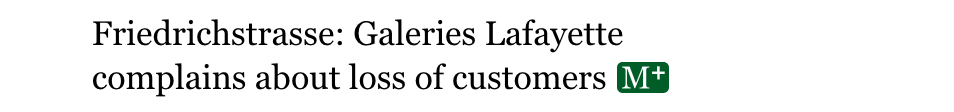
\includegraphics[height=0.11\textwidth,keepaspectratio=true]{../04-figures/08/10-lafayette1}
    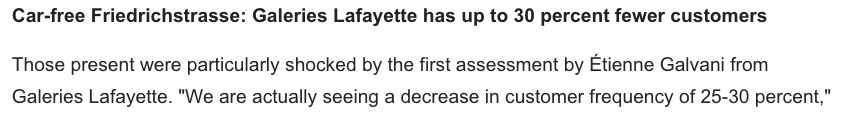
\includegraphics[height=0.125\textwidth,keepaspectratio=true]{../04-figures/08/11-lafayette2}
    \end{figure} \scriptsize
    Note: Car traffic was banned from parts of Friedrichstra{\ss}e from 29 August onwards
\end{frame}


\begin{frame}
	\frametitle{Friedrichstra{\ss}e}
	\begin{enumerate}
		\item What is problematic about the claim by the Lafayette spokesperson? 
		\item How would you go about evaluating the claim that the road closure led to a reduction in consumer traffic?
		\item What data would you collect (DV, IV, covariates)?
		\item How would the data need to look like to make the claim credible?
	\end{enumerate}
\end{frame}



\begin{frame}
	\frametitle{Abadie and Gardeazabal \citeyear{abadie_economic_2003}}
	\begin{enumerate}
		\item What is the research question?
		\item How credible is their claim?
		\item What would be an alternative approach to using the synthetic control method?
	\end{enumerate}
\end{frame}


\begin{frame}
	\frametitle{Abadie and Gardeazabal \citeyear{abadie_economic_2003}: Credibility}
	\footnotesize
	Diverging trends in control units: ``During 1990-1997 Catalonia outperformed the synthetic control by around 4 percent in per capita GDP.'' (p119)
	
	Parallel process in treatment group: ``In fact, the industrial share of GDP declined 17 percentage points (from 45 percent to 28 percent) for the Basque Country during the 1964-1993 period. The industrial share of
the GDP decreased 15 percentage points (from 38 percent to 23 percent) for the synthetic control during the same period.'' (p121)

\end{frame}


\begin{frame}
	\frametitle{Abadie and Gardeazabal \citeyear{abadie_economic_2003}: Credibility}
	\footnotesize
    But: Out-of-sample example plausibility probe
  	 \begin{figure} 
    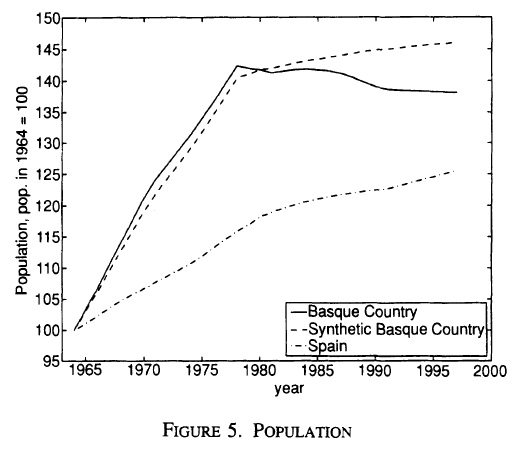
\includegraphics[height=.65\textheight,keepaspectratio=true]{../04-figures/08/12-ag_fig5}
    \end{figure} \scriptsize
\end{frame}



\begin{frame}
	\frametitle{Abadie and Gardeazabal \citeyear{abadie_economic_2003}}
	Possible alternative strategies
	
	Move down to province or municipality level to enlarge sample size, then 
	\begin{enumerate}
		\item DiD
		\item Matching
		\item Matching + DiD
		\item other ideas?
	\end{enumerate}
\end{frame}


% END
\begin{frame}
\begin{center}
    \LARGE Thank you for watching, and see you next Monday!
\end{center}
\end{frame}

% REFERENCES %

\begin{frame}[allowframebreaks]
\frametitle{References}
\bibliographystyle{apacite}
\scriptsize\bibliography{../Bibliography}
\end{frame}

\end{document}
